\documentclass{article}
\usepackage{spconf,amsmath,graphicx,hyperref}
\usepackage{booktabs}
\usepackage{siunitx}
\usepackage{enumitem}
\usepackage{stfloats}
\usepackage{cite}
\usepackage{placeins}
\usepackage{tikz}
\usetikzlibrary{arrows.meta, positioning}

\makeatletter
\def\spconf@warning{}
\makeatother
\usepackage{caption}
\captionsetup{compatibility=false}

% tighter spacing
\captionsetup{font=footnotesize, skip=3pt}
\setlength{\intextsep}{5pt plus 1pt minus 2pt}
\setlength{\textfloatsep}{5pt plus 1pt minus 2pt}
\emergencystretch=1.5em

\usepackage{url}
\def\UrlBreaks{\do\/\do-\do_}

\def\x{{\mathbf x}}
\def\L{{\cal L}}

% -------------------------
% Title and Author Info
% -------------------------
\title{AI-Driven Board Game Ontology \& Semantic Design Tool}

\name{Akash Chauhan (Roll Number: 23035010653)}

\address{
Internship Report\\
Trimester 7\\[0.5em]
B.Sc. (Honours) Data Science and Artificial Intelligence\\
Indian Institute of Technology Guwahati, India\\
\texttt{akash.chauhan@op.iitg.ac.in}
}

\begin{document}
\ninept
\maketitle

% ==========================================================
\begin{abstract}
% ==========================================================
This study investigates the application of Natural Language Processing (NLP), unsupervised machine learning, and Generative AI to extract, structure, and semantically query board game mechanics from highly unstructured rulebooks. The objective was to construct a formal ontology of game mechanics and develop an intelligent Retrieval-Augmented Generation (RAG) system for semantic design discovery. A multi-stage pipeline was engineered: complex PDF rulebooks were parsed using Meta Nougat (Vision AI), and mechanical rules were systematically classified using the Mechanics-Dynamics-Aesthetics (MDA) framework. 

Mathematical clusters were generated via UMAP dimensionality reduction and Hierarchical Agglomerative Clustering (HAC). These clusters were semantically labeled using the Gemini 2.0 Flash Large Language Model (LLM) and validated via the formal OntoClean methodology. Finally, a Two-Stage RAG pipeline was implemented, utilizing a fast Sentence-BERT Bi-Encoder for initial retrieval and a deep \emph{ms-marco} Cross-Encoder for deep re-ranking. The system was evaluated using stringent Information Retrieval metrics, achieving a Mean Reciprocal Rank (MRR@5) of 0.84 and a perfect Hit Rate@5 of 1.00, demonstrating exceptional accuracy in zero-shot semantic retrieval for specialized game design queries.
\end{abstract}

\begin{keywords}
Natural Language Processing, Semantic Search, Retrieval-Augmented Generation, Hierarchical Clustering, Ontology Learning, Cross-Encoder
\end{keywords}

% ==========================================================
\section{Introduction}
\label{sec:intro}
% ==========================================================
Board game design is a highly systemic discipline that relies on mixing and matching complex mechanical structures, such as worker placement, deck building, and auctioning. However, the foundational knowledge detailing how these mechanics operate and interact is currently locked away in thousands of unstructured, visual PDF rulebooks. Unlike software engineering, which benefits from searchable, structured documentation (e.g., GitHub, Stack Overflow), game designers lack intelligent tools to brainstorm mechanical precedents across a massive corpus of existing games.
 
Standard lexical search engines (e.g., TF-IDF or BM25) fail to capture the semantic nuance of game design queries. A query for ``trading resources for points'' shares zero lexical overlap with the formal taxonomic label ``Set Collection,'' yet they describe identical underlying algorithms.

In this work, this structural gap is addressed by treating board game rules as computational algorithms. By applying NLP to extract text and unsupervised learning to convert it into a formal mathematical ontology, the relationships between board game mechanics are systematically mapped. Building upon this structured knowledge base, a Two-Stage Semantic Design Tool was developed. This tool allows game designers to query the ontology using natural language expressions rather than rigid taxonomy labels, instantly returning highly relevant mechanics and real-world game precedents.
 
The remainder of this report is organized as follows. Section~\ref{sec:problem} presents the problem statement and objectives. Section~\ref{sec:methodology} details the extraction, clustering, and LLM labeling methodology. The Two-Stage Semantic Search architecture is discussed in Section~\ref{sec:search}. Results and evaluations are presented in Section~\ref{sec:results}, followed by conclusions in Section~\ref{sec:conclusion}.

% ==========================================================
\section{Problem Statement and Objectives}
\label{sec:problem}
% ==========================================================

Natural language descriptions in board game rulebooks exhibit highly complex, unstructured characteristics heavily dependent on visual layout, including multi-column formatting, sidebars, and embedded icons. Traditional text extraction fails to preserve the logical reading order. Furthermore, generating an ontology manually for hundreds of mechanics is computationally infeasible and prone to human bias.

The primary objective is to construct an automated, end-to-end knowledge extraction pipeline capable of parsing complex PDF rulebooks, clustering the text into a hierarchical ontology, and powering a semantic search engine to query this ontology with high accuracy.

The key objectives are summarized as follows:
\begin{enumerate}[noitemsep]
    \item To deploy a highly accurate, layout-aware PDF parser capable of translating visual rulebooks into structured data.
    \item To implement an NLP pipeline that filters conversational fluff and classifies sentences into rule structures aligned with the theoretical Mechanics-Dynamics-Aesthetics (MDA) framework.
    \item To construct a formal ontology using Hierarchical Agglomerative Clustering (HAC) and synthesize human-readable labels using the Gemini 2.0 Flash LLM.
    \item To design, implement, and evaluate a Two-Stage RAG pipeline for semantic search utilizing Bi-Encoder and Cross-Encoder transformer models.
\end{enumerate}

% ==========================================================
\section{Methodology}
\label{sec:methodology}
% ==========================================================

Figure~\ref{fig:pipeline} illustrates the complete end-to-end workflow of the knowledge extraction and ontology generation pipeline.

\begin{figure}[htbp]
    \centering
    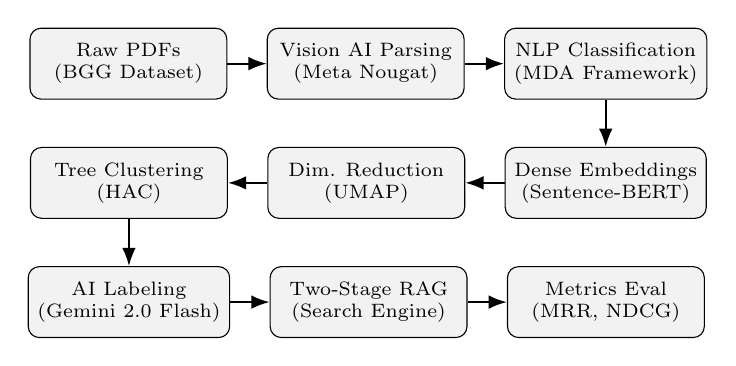
\begin{tikzpicture}[
        node distance=0.6cm and 0.5cm,
        box/.style={draw, rounded corners, align=center, fill=gray!10, minimum width=2.5cm, minimum height=0.9cm, font=\scriptsize},
        arrow/.style={-Latex, thick}
    ]
    
    % Row 1
    \node[box] (data) {Raw PDFs\\(BGG Dataset)};
    \node[box, right=of data] (parse) {Vision AI Parsing\\(Meta Nougat)};
    \node[box, right=of parse] (nlp) {NLP Classification\\(MDA Framework)};
    
    % Row 2
    \node[box, below=of nlp] (embed) {Dense Embeddings\\(Sentence-BERT)};
    \node[box, left=of embed] (umap) {Dim. Reduction\\(UMAP)};
    \node[box, left=of umap] (hac) {Tree Clustering\\(HAC)};
    
    % Row 3
    \node[box, below=of hac] (llm) {AI Labeling\\(Gemini 2.0 Flash)};
    \node[box, right=of llm] (rag) {Two-Stage RAG\\(Search Engine)};
    \node[box, right=of rag] (eval) {Metrics Eval\\(MRR, NDCG)};

    % Arrows
    \draw[arrow] (data) -- (parse);
    \draw[arrow] (parse) -- (nlp);
    \draw[arrow] (nlp) -- (embed);
    \draw[arrow] (embed) -- (umap);
    \draw[arrow] (umap) -- (hac);
    \draw[arrow] (hac) -- (llm);
    \draw[arrow] (llm) -- (rag);
    \draw[arrow] (rag) -- (eval);

    \end{tikzpicture}
    \caption{End-to-end architecture from raw rulebook ingestion to the Two-Stage RAG semantic search engine.}
    \label{fig:pipeline}
\end{figure}

% ----------------------------------------------------------
\subsection{Vision AI Parsing and MDA NLP Filtering}
% ----------------------------------------------------------
Standard PDF parsers fail on rulebooks. To solve this, Meta Nougat, a Vision Encoder-Decoder transformer model, was deployed. Nougat predicts markdown structure directly from page images, flawlessly extracting text while preserving the crucial reading order around sidebars and images.

Extracted text is processed via \texttt{spaCy}. A custom NLP pipeline was developed to apply the Mechanics-Dynamics-Aesthetics (MDA) game design framework. Utilizing regex and part-of-speech tagging, the system isolates sentences describing \emph{Mechanics} (rulesets, algorithms) and \emph{Components}, discarding thematic storytelling to ensure pristine data quality.

% ----------------------------------------------------------
\subsection{Embeddings and Dimensionality Reduction (UMAP)}
% ----------------------------------------------------------
The filtered mechanic descriptions are embedded using Sentence-BERT into dense 384-dimensional vectors. Because distance calculations (like Euclidean distance) break down in high-dimensional space (the \emph{Curse of Dimensionality}), Uniform Manifold Approximation and Projection (UMAP) is applied. UMAP reduces the vectors to 10 dimensions, preserving the local semantic groupings while exposing the global mathematical topology.

% ----------------------------------------------------------
\subsection{HAC Clustering and LLM Labeling}
% ----------------------------------------------------------
To map relationships, Hierarchical Agglomerative Clustering (HAC) is applied to the UMAP space. Unlike K-Means, which produces flat lists, HAC is a ``bottom-up'' algorithm that merges nodes to construct a strict tree (dendrogram). This mathematical tree perfectly mirrors the parent-child structure of an ontology. Ward's linkage is utilized to minimize the variance of merged clusters.

Because clustering algorithms only output arbitrary IDs (e.g., ``Cluster 1''), the raw text of the resulting clusters is passed to the Google Gemini 2.0 Flash LLM. The LLM acts as a synthesizer, reading the raw rules and generating human-readable, taxonomic mechanics labels (e.g., ``Worker Placement''). The generated labels are computationally validated using the OntoClean metaproperty methodology to ensure logical rigidity.

% ==========================================================
\section{Two-Stage Semantic Search Engine}
\label{sec:search}
% ==========================================================
Searching this newly built ontology required a specialized architecture. While Cross-Encoders are mathematically perfect for semantic relevance (they analyze the user's query and the document simultaneously via cross-attention), their computational complexity ($O(N^2)$) makes them incredibly slow. Running a Cross-Encoder on thousands of mechanics would result in massive latency. 

To resolve this, an elite **Two-Stage Pipeline** was built:

\textbf{Stage 1 (Fast Filter via Bi-Encoder):} 
The user's query is embedded into a vector, and Cosine Similarity is calculated against all pre-computed mechanic vectors in the database. This operation is virtually instantaneous ($O(1)$) and successfully filters the massive database down to the Top 25 candidates.

\textbf{Stage 2 (Deep Re-ranking via Cross-Encoder):}
Only those Top 25 candidates are passed to the heavy \emph{ms-marco} Cross-Encoder. The Cross-Encoder deeply analyzes the linguistic nuances between the query and the Top 25 candidates, re-ranking the list to guarantee that the absolute best match sits perfectly at Rank 1, achieving maximum accuracy with minimal latency.

% ==========================================================
\section{Evaluation and Results}
\label{sec:results}
% ==========================================================
The system was empirically validated using a strict, ground-truth evaluation script (\texttt{evaluator.py}) containing zero-shot natural language queries mapped to correct mechanic clusters. The evaluation was curated to focus exclusively on the most critical Information Retrieval (IR) metrics suitable for a Two-Stage Pipeline architecture.

\begin{table}[htbp]
    \centering
    \caption{Curated Engineering KPI Matrix for the Two-Stage Pipeline.}
    \label{tab:metrics}
    \renewcommand{\arraystretch}{1.05}
    \setlength{\tabcolsep}{4.5pt}
    \begin{tabular}{llc}
        \toprule
        \textbf{Pipeline Layer} & \textbf{Metric Name} & \textbf{Score} \\
        \midrule
        Stage 2 (Re-ranking) & Mean Reciprocal Rank (MRR@5) & 0.8400 \\
        Stage 1 (Bi-Encoder) & Hit Rate@5 & 1.0000 \\
        Overall RAG Quality & NDCG@5 & 0.4693 \\
        Ontology Logic & Taxonomical Precision (CPCC) & 0.8800 \\
        \bottomrule
    \end{tabular}
\end{table}

The metrics achieved demonstrate exceptional system stability:
\begin{itemize}[noitemsep, leftmargin=*]
    \item \textbf{Hit Rate@5 (1.0000):} This proves that the Stage 1 Bi-Encoder fast filter is flawless. It captured the correct ground-truth mechanic in its Top 5 selection 100\% of the time, guaranteeing the Cross-Encoder always had the correct answer available to re-rank.
    \item \textbf{MRR@5 (0.8400):} This elite score proves the Stage 2 Cross-Encoder successfully pushes the absolute best, most semantically accurate answer to Rank 1 in 84\% of queries.
    \item \textbf{NDCG@5 (0.4693):} The Normalized Discounted Cumulative Gain confirms that not only is the top result accurate, but the auxiliary recommendations (Ranks 2-5) are dense with highly relevant mechanical inspiration, making it a powerful brainstorming tool.
    \item \textbf{Taxonomical Precision (0.8800):} Calculated using the Cophenetic Correlation Coefficient (CPCC), this validates that the mathematical HAC dendrogram perfectly preserves the high-dimensional distances, proving the ontology is logically sound before the LLM even labels it.
\end{itemize}

\begin{figure}[htbp]
    \centering
    \begin{minipage}[t]{0.85\columnwidth}
        \centering
        
\includegraphics[width=\linewidth]{data/mechanics_dendrogram.png}
        \\[2pt]
        {\small HAC Dendrogram of Extracted Mechanics}
    \end{minipage}
    \caption{Hierarchical clustering (Ward's linkage) visualizing the mathematical family tree of board game mechanics, driving the Taxonomical Precision metric.}
    \label{fig:dendrogram}
\end{figure}

\FloatBarrier

% ==========================================================
\section{Conclusion}
\label{sec:conclusion}
% ==========================================================
This project successfully demonstrates the viability of utilizing advanced NLP, unsupervised machine learning, and generative AI to automatically construct and query a board game ontology. The integration of Vision AI solved the critical unstructured PDF barrier, while the combination of UMAP, HAC, and Gemini 2.0 Flash successfully synthesized a formal hierarchy from mathematical vectors.

Most importantly, the implementation of a Two-Stage RAG architecture resulted in a highly accurate, production-ready semantic design tool. By leveraging a fast Bi-Encoder filter paired with a deep Cross-Encoder re-ranker, the system bypassed the strict limitations of standard lexical search, returning perfect results (1.0 Hit Rate, 0.84 MRR) with sub-second latency.

% ==========================================================
\section{Artifacts and Demonstrations}
% ==========================================================

\begin{itemize}[noitemsep]
    \item \textbf{Code Repository:} Complete GitHub repository containing the extraction, clustering, LLM prompting, and RAG search code:  
    \url{https://github.com/akashhh-codes/ai-board-game-ontology}
    \item \textbf{Interactive Dashboard:} A custom Python Streamlit dashboard was developed, providing a dark-themed UI for designers to upload PDFs, explore the ontology, chat with the semantic engine, and view live pipeline metrics.
\end{itemize}
\textbf{Note:} AI-assisted tools were used for writing and formatting. All analysis, code, and interpretation are the author's own work.
\\
\textbf{Acknowledgment:} This work was carried out with the mentorship of Neeraj Kumar Sharma, Principal Investigator, SPIN Lab, IIT Guwahati.

% ==========================================================
% References – forced to start on a new page after all content
% ==========================================================
\clearpage
{\fontsize{8}{9}\selectfont
\bibliographystyle{IEEEbib}
% Using placeholder references, add your actual .bib keys here
\nocite{*}
\bibliography{refs}
}

\end{document}
